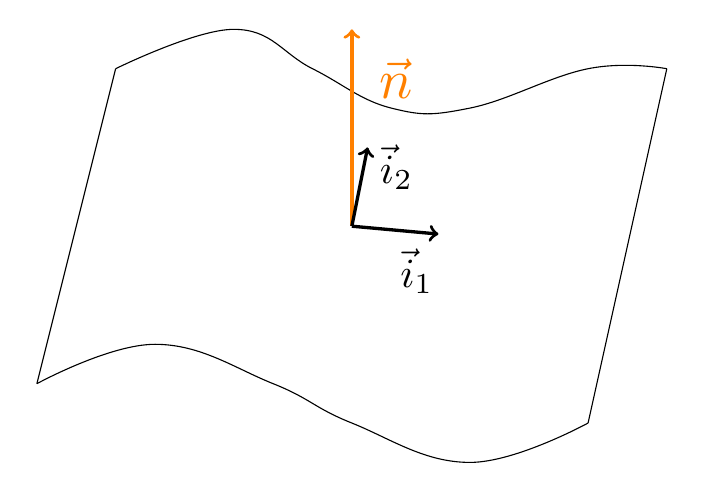
\begin{tikzpicture}

\draw (-1,1.5) node (v2) {} -- (-2,-2.5) node (v1) {};
\draw (6,1.5) node (v3) {} -- (5,-3);
\draw  plot[smooth, tension=.7] coordinates {(v1) (-0.5,-2) (1,-2.5) (2,-3) (3.5,-3.5) (5,-3)};


\draw  plot[smooth, tension=.7] coordinates {(v2) (0.5,2) (1.5,1.5) (2.5,1) (3.5,1) (5,1.5) (v3)};
\draw [->, very thick, orange] (2,-0.5) node (v4) {} -- (2,2) node [orange, near end, right=2, scale=2] {$\vec{n}$};
\draw [->, very thick] (2,-0.5) -- (2.2,0.5) node [black, near end, right, scale=1.5] {$\vec{i}_2$};
\draw [->, very thick] (2,-0.5) -- (3.1,-0.6) node [black, near end, below, scale=1.5] {$\vec{i}_1$};
\end{tikzpicture}